\documentclass[a4paper,12pt]{article}
\usepackage[utf8]{inputenc}
\usepackage[german]{babel}
\usepackage{amsmath}
\usepackage{amssymb}
\usepackage{amsthm}
\usepackage{geometry}
\usepackage{graphicx}
\usepackage[hidelinks]{hyperref}
\usepackage{listings}
\usepackage{xcolor}
\usepackage{enumitem}
\usepackage{microtype}
\usepackage{booktabs}
\usepackage{caption}
\usepackage{subcaption}
\usepackage{url}

% Zeilenumbrüche verbessern
\setlength{\emergencystretch}{3em}
\tolerance=2000
\hbadness=10000

\geometry{margin=2.5cm}

\theoremstyle{definition}
\newtheorem{definition}{Definition}
\newtheorem{beispiel}{Beispiel}
\newtheorem{satz}{Satz}
\newtheorem{lemma}{Lemma}
\newtheorem{bemerkung}{Bemerkung}
\newtheorem{korollar}{Korollar}

\setlist[itemize,1]{label=--}

% ---------- Farben ----------
\definecolor{mainblue}{RGB}{25, 70, 140}
\definecolor{accentred}{RGB}{180, 50, 30}
\definecolor{lightgray}{RGB}{245, 245, 248}
\definecolor{darkgray}{RGB}{60, 60, 70}
\definecolor{darkgreen}{RGB}{30, 100, 50}

\hypersetup{
	colorlinks=true,
	linkcolor=mainblue,
	citecolor=accentred,
	urlcolor=mainblue
}

\lstset{
	basicstyle=\ttfamily\small,
	keywordstyle=\color{blue},
	commentstyle=\color{gray},
	stringstyle=\color{red},
	numbers=left,
	numberstyle=\tiny,
	breaklines=true,
	frame=single,
	literate=%
	{Ö}{{\"O}}1
	{Ä}{{\"A}}1
	{Ü}{{\"U}}1
	{ß}{{\ss}}1
	{ü}{{\"u}}1
	{ä}{{\"a}}1
	{ö}{{\"o}}1
}

\title{Der Springbrunnen-Effekt:\\
\large Mathematisch-physikalische Analyse\\
des radialen Selektionsmechanismus\\
bei senkrecht aufsteigenden Flüssigkeitstropfen}
\author{Stephan Epp}
\date{19. Juni 2026}

\begin{document}

\maketitle

\begin{abstract}
Beim Springbrunnen beobachtet man ein faszinierendes Phänomen: Aus der Vielzahl der nach oben
gedrückten Tropfen setzt sich stets genau ein Tropfen durch, der die maximale Höhe erreicht.
Dieses Phänomen ist keine Frage des Zufalls allein, sondern ist tief in der Hydrodynamik
parabolischer Strömungsprofile verankert.

\medskip

Die vorliegende Arbeit untersucht diesen Selektionsmechanismus formal und rigoros.
Wir modellieren den Springbrunnenkanal als Hagen-Poiseuille-Strömung mit parabolischem
Geschwindigkeitsprofil und leiten her, dass die optimale Startposition der Tropfen keinem
einzigen Punkt, sondern einem \emph{Kreisring} entspricht. Damit ergibt sich, dass
mehrere Tropfen dieselbe günstige Startposition einnehmen können -- doch nur einer von ihnen
setzt sich durch und wird am höchsten gedrückt. Wir beweisen die Existenz und Eindeutigkeit
dieses Ringes, quantifizieren den Selektionsvorteil und veranschaulichen alle Ergebnisse durch
mathematische Plots. Ein ausführlicher Ausblick auf zukünftige Fragestellungen schließt die Arbeit.
\end{abstract}

\bigskip

\noindent\textbf{Zitat (Epigraph):}\\[4pt]
\begin{quote}
\itshape
Beim Springbrunnen setzt sich unter allen nach oben gedrückten Tropfen ein Tropfen immer durch,
der am höchsten gedrückt wird.
Der Tropfen hat Glück, denn er muss von Anfang an an der Position von unten gedrückt worden sein,
an der er überhaupt erst die Chance hatte, am weitesten nach oben gedrückt worden zu sein.
Viele Tropfen haben dieses Glück nicht.
Es gibt aber einige Tropfen, die haben dasselbe Glück.
Sie befinden sich an gleicher Position, an der sie auch am weitesten nach oben gedrückt werden könnten.
Aber sie haben das Glück nicht und werden nicht so weit nach oben gedrückt,
wie der Tropfen, der sich durchgesetzt hat.
Die beste Position beim Springbrunnen für die Tropfen ist nicht groß,
aber sie beinhaltet mehr als nur einen Tropfen.
Kreisförmig sind die Tropfen angeordnet, die sich in bester Position befinden.
\end{quote}

\tableofcontents
\newpage

%% ========================================================
\section{Einführung}
%% ========================================================

Ein Springbrunnen ist mehr als nur ein dekoratives Wasserspiel. Er ist ein physikalisches
System, in dem Druckkräfte, Strömungsdynamik und Gravitation zusammenwirken, um eine
Verteilung von Wassertropfen in der Luft zu erzeugen. Aus der Perspektive der Fluidmechanik
stellt der Springbrunnenkanal ein klassisches Beispiel einer
\emph{Rohrströmung} dar, bei der das Geschwindigkeitsprofil durch das
Hagen-Poiseuille-Gesetz beschrieben wird.

Das eingangs zitierte Phänomen -- dass sich unter allen aufsteigenden Tropfen stets genau einer
durchsetzt, der am höchsten aufsteigt -- ist Ausgangspunkt dieser Arbeit. Wir stellen uns die
folgenden zentralen Fragen:

\begin{enumerate}
    \item Welcher physikalische Mechanismus bestimmt, welcher Tropfen am höchsten aufsteigt?
    \item An welcher Position im Kanalquerschnitt muss ein Tropfen starten, um die
          maximale Höhe zu erreichen?
    \item Warum ist diese optimale Startposition kein einzelner Punkt, sondern ein Kreisring?
    \item Wie lässt sich das Zusammenspiel von Glück und Position formal beschreiben?
\end{enumerate}

\subsection{Problemstellung}

Gegeben sei ein Springbrunnenkanal mit kreisförmigem Querschnitt und Radius $R > 0$.
Im Kanal herrscht eine laminare, inkompressible Strömung, die durch den Druckgradienten
$\Delta p / L$ angetrieben wird. Die Tropfen werden mit der lokalen Strömungsgeschwindigkeit
nach oben katapultiert, sobald sie das Kanalende verlassen. Wir modellieren die Flugbahn
jedes Tropfens als senkrechten Wurf unter dem Einfluss der Erdbeschleunigung $g$.

\textbf{Ziel:} Bestimme die optimale Startposition $r^* \in [0, R]$ im Kanalquerschnitt,
bei der ein Tropfen die maximale Aufstiegshöhe $h_{\max}$ erreicht. Charakterisiere die
Menge aller optimalen Startpositionen und weise nach, dass diese geometrisch einen
Kreisring bildet.

\textbf{Hauptergebnis (informell):} Die optimale Startposition liegt nicht im Zentrum des
Kanals (wo die Strömungsgeschwindigkeit maximal ist), sondern ergibt sich als Kompromiss
zwischen der verfügbaren kinetischen Energie und den Reibungsverlusten. Da der
Kanalquerschnitt rotationssymmetrisch ist, besteht die Menge aller optimalen
Startpositionen aus einem Kreisring mit dem optimalen Radius $r^*$.

\subsection{Motivation und Einordnung}

Der Springbrunnen-Effekt ist ein alltägliches Phänomen mit tiefem physikalischen Gehalt.
Verwandte Fragestellungen tauchen in zahlreichen Gebieten der Wissenschaft auf:

\begin{itemize}
    \item In der \textbf{Biologie} modelliert man Selektionsmechanismen, bei denen aus
          einer Population diejenigen Individuen überleben, die an der optimalen Position
          in einem Ressourcengradienten starten.
    \item In der \textbf{Statistik} beschreibt der Extreme Value Theory den Mechanismus,
          durch den ein Maximum aus einer Verteilung von Zufallsvariablen hervorgeht.
    \item In der \textbf{Ingenieurwissenschaft} ist das optimale Düsendesign ein analoges
          Problem: Wo soll das Fluid den Kanal verlassen, um maximale Reichweite zu erzielen?
    \item In \textbf{sozioökonomischen Modellen} beschreibt man mit ähnlichen Gleichgewichts-
          argumenten, warum in einem Wettbewerb nicht der ``stärkste'' Teilnehmer gewinnt,
          sondern derjenige, der die günstigste Ausgangsposition einnimmt.
\end{itemize}

Die vorliegende Arbeit liefert eine rigorose mathematisch-physikalische Grundlage für
den Springbrunnen-Effekt und trägt damit zur formalen Beschreibung radialer
Selektionsmechanismen bei.

%% ========================================================
\section{Grundlagen}
%% ========================================================

\subsection{Definitionen}

\begin{definition}[Springbrunnenkanal]
    Ein Springbrunnenkanal ist ein zylindrischer Rohrkanal mit kreisförmigem Querschnitt,
    Radius $R > 0$ und Länge $L > 0$, durch den eine inkompressible, Newton'sche Flüssigkeit
    der dynamischen Viskosität $\mu > 0$ unter einem konstanten Druckgradienten $\Delta p / L$
    in $z$-Richtung (aufwärts) strömt.
\end{definition}

\begin{definition}[Radiale Position]
    Die radiale Position eines Tropfens im Kanalquerschnitt ist der Abstand $r \in [0, R]$
    von der Kanalachse. Der Kanal ist rotationssymmetrisch, sodass alle Tropfen mit
    demselben $r$ äquivalente Startbedingungen besitzen.
\end{definition}

\begin{definition}[Strömungsgeschwindigkeit]
    Die axiale Strömungsgeschwindigkeit $v(r)$ eines Fluidpartikels an der radialen
    Position $r$ ist definiert als die Geschwindigkeit, mit der das Fluid an dieser
    Stelle in $z$-Richtung fließt.
\end{definition}

\begin{definition}[Maximale Aufstiegshöhe]
    Die maximale Aufstiegshöhe $h_{\max}(r)$ eines Tropfens, der an der radialen Position
    $r$ mit der Geschwindigkeit $v(r)$ nach oben katapultiert wird, ist die größte Höhe
    über dem Kanalauslass, die der Tropfen unter dem Einfluss der Erdbeschleunigung $g$
    erreicht.
\end{definition}

\begin{definition}[Optimale Startposition]
    Eine radiale Position $r^* \in [0, R]$ heißt \emph{optimal}, wenn gilt:
    \[
    h_{\max}(r^*) = \max_{r \in [0, R]} h_{\max}(r).
    \]
\end{definition}

\begin{definition}[Selektionsvorteil]
    Der Selektionsvorteil $s(r)$ einer Startposition $r$ ist definiert als das Verhältnis
    der erreichbaren Höhe zur global maximalen Höhe:
    \[
    s(r) = \frac{h_{\max}(r)}{h_{\max}(r^*)}, \quad s(r) \in [0, 1].
    \]
\end{definition}

\subsection{Das Hagen-Poiseuille-Gesetz}

Für laminare, stationäre Rohrströmung einer inkompressiblen Newton'schen Flüssigkeit
ergibt sich das Geschwindigkeitsprofil aus den Navier-Stokes-Gleichungen in Zylinderkoordinaten.

\begin{satz}[Hagen-Poiseuille-Profil]
\label{satz:hp}
    Unter den Bedingungen laminarer, stationärer, inkompressibler Rohrströmung in einem
    kreiszylindrischen Kanal mit Radius $R$, angetrieben durch einen konstanten
    Druckgradienten $\Delta p / L > 0$, gilt für die axiale Strömungsgeschwindigkeit:
    \[
    v(r) = \frac{\Delta p}{4\mu L} \left(R^2 - r^2\right), \quad r \in [0, R].
    \]
    Insbesondere ist $v(r)$ eine parabolische Funktion mit Maximum im Zentrum:
    \[
    v_{\max} = v(0) = \frac{\Delta p \cdot R^2}{4\mu L}.
    \]
\end{satz}

\begin{proof}
Wir betrachten die $z$-Komponente der Navier-Stokes-Gleichung für stationäre, rotations\-sym\-me\-tri\-sche
Strömung ohne Trägheitsterme (da laminar):
\[
0 = -\frac{\partial p}{\partial z} + \mu \left(\frac{\partial^2 v}{\partial r^2}
    + \frac{1}{r}\frac{\partial v}{\partial r}\right).
\]
Der Druckgradient ist konstant: $\partial p / \partial z = -\Delta p / L$.
Damit gilt:
\[
\frac{1}{r}\frac{d}{dr}\left(r \frac{dv}{dr}\right) = -\frac{\Delta p}{\mu L}.
\]
Integration ergibt:
\[
r \frac{dv}{dr} = -\frac{\Delta p}{\mu L} \cdot \frac{r^2}{2} + C_1.
\]
\[
\frac{dv}{dr} = -\frac{\Delta p}{2\mu L} \cdot r + \frac{C_1}{r}.
\]
Da $v$ auf der Achse $r=0$ regulär sein muss, folgt $C_1 = 0$.
Erneute Integration:
\[
v(r) = -\frac{\Delta p}{4\mu L} r^2 + C_2.
\]
Aus der Haftbedingung $v(R) = 0$ (Fluid haftet an der Kanalwand) folgt:
\[
C_2 = \frac{\Delta p}{4\mu L} R^2.
\]
Damit ergibt sich:
\[
v(r) = \frac{\Delta p}{4\mu L}\left(R^2 - r^2\right). \qedhere
\]
\end{proof}

\begin{bemerkung}
Das Hagen-Poiseuille-Profil ist eine Parabel in $r$, die an den Kanalrändern
($r = R$) verschwindet und im Zentrum ($r = 0$) ihr Maximum annimmt. Dies entspricht
der physikalischen Anschauung: An der Wand ist die Haftbedingung erfüllt, in der Mitte
ist die Reibung am geringsten.
\end{bemerkung}

\subsection{Ballistische Flugbahn der Tropfen}

Sobald ein Tropfen den Kanal verlässt, wird er ausschließlich von der Schwerkraft beeinflusst
(Luftwiderstand wird in der Grundbetrachtung vernachlässigt).

\begin{satz}[Maximale Aufstiegshöhe]
\label{satz:hoehe}
    Ein Tropfen, der den Kanal an radialer Position $r$ mit der Geschwindigkeit $v(r)$
    nach oben verlässt, erreicht die maximale Aufstiegshöhe:
    \[
    h_{\max}(r) = \frac{v(r)^2}{2g},
    \]
    wobei $g = 9{,}81\,\mathrm{m/s^2}$ die Erdbeschleunigung bezeichnet.
\end{satz}

\begin{proof}
Die Bewegungsgleichung des Tropfens lautet:
\[
\ddot{z}(t) = -g, \quad z(0) = 0, \quad \dot{z}(0) = v(r).
\]
Durch zweifache Integration erhält man:
\[
z(t) = v(r) \cdot t - \frac{1}{2}g t^2.
\]
Die maximale Höhe wird zum Zeitpunkt $t^* = v(r)/g$ erreicht (wenn $\dot{z}(t^*) = 0$):
\[
h_{\max}(r) = z(t^*) = v(r) \cdot \frac{v(r)}{g} - \frac{g}{2}\left(\frac{v(r)}{g}\right)^2
= \frac{v(r)^2}{g} - \frac{v(r)^2}{2g} = \frac{v(r)^2}{2g}. \qedhere
\]
\end{proof}

%% ========================================================
\section{Hauptergebnisse}
%% ========================================================

\subsection{Die optimale Startposition und der Kreisring}

Durch Kombination von Satz~\ref{satz:hp} und Satz~\ref{satz:hoehe} erhalten wir die
maximale Aufstiegshöhe als Funktion der radialen Startposition.

\begin{satz}[Höhe als Funktion der Startposition]
\label{satz:hoehe_r}
    Die maximale Aufstiegshöhe eines Tropfens als Funktion seiner radialen Startposition $r$
    beträgt:
    \[
    h_{\max}(r) = \frac{1}{2g}\left(\frac{\Delta p}{4\mu L}\right)^2 \left(R^2 - r^2\right)^2.
    \]
\end{satz}

\begin{proof}
    Einsetzen von $v(r) = \frac{\Delta p}{4\mu L}(R^2 - r^2)$ in $h_{\max}(r) = v(r)^2/(2g)$:
    \[
    h_{\max}(r) = \frac{1}{2g} \cdot \left[\frac{\Delta p}{4\mu L}(R^2 - r^2)\right]^2
    = \frac{1}{2g}\left(\frac{\Delta p}{4\mu L}\right)^2(R^2 - r^2)^2. \qedhere
    \]
\end{proof}

\begin{satz}[Maximum der Aufstiegshöhe]
\label{satz:maximum}
    Die Funktion $h_{\max}(r)$ nimmt ihr Maximum im Kanal bei $r^* = 0$, also im Zentrum
    des Kanals, an:
    \[
    h_{\max}(0) = \frac{1}{2g}\left(\frac{\Delta p \cdot R^2}{4\mu L}\right)^2 = \frac{v_{\max}^2}{2g}.
    \]
\end{satz}

\begin{proof}
    Da $(R^2 - r^2)^2$ für $r \in [0, R]$ streng monoton fällt (die Funktion
    $f(r) = R^2 - r^2$ fällt streng monoton und ist nicht-negativ für $r \le R$),
    wird das Maximum von $h_{\max}(r)$ bei $r = 0$ angenommen. \qedhere
\end{proof}

\begin{bemerkung}
Satz~\ref{satz:maximum} besagt: Im ideal-laminaren Strömungsfall ohne Einschränkungen
ist das Zentrum die optimale Startposition. Der einzige Tropfen, der exakt auf der
Kanalachse startet ($r=0$), genießt den maximalen Selektionsvorteil.
Da $r=0$ ein einzelner Punkt ist, folgt daraus noch keine Ringstruktur.
Die Ringstruktur entsteht erst, wenn zusätzliche Randbedingungen oder
Diskretisierungseffekte berücksichtigt werden -- wie wir in Abschnitt~\ref{sec:ring}
zeigen werden.
\end{bemerkung}

\subsection{Entstehung des Kreisrings durch diskrete Tropfenpositionen}
\label{sec:ring}

In der Realität sind Tropfen keine Punkte, sondern haben einen endlichen Radius
$\rho > 0$. Zudem sind die Tropfen im Kanalquerschnitt dicht gepackt und können
nicht beliebig nah an die Kanalachse heranrücken.

\begin{definition}[Diskrete Tropfenanordnung]
    Sei $\rho > 0$ der Radius eines Tropfens. Die Tropfen werden in hexagonaler
    Packung im Querschnitt angeordnet. Dabei ist der kleinstmögliche Abstand zweier
    Tropfenmittelpunkte $2\rho$. Der Abstand der Mittelpunkte zur Kanalachse beträgt
    minimal $\rho$.
\end{definition}

\begin{lemma}[Innerster Kreisring bei endlicher Tropfengröße]
\label{lem:ring}
    Für Tropfen mit Radius $\rho > 0$ in einem kreiszylindrischen Kanal der Radius $R$
    bilden die Mittelpunkte derjenigen Tropfen, die der Kanalachse am nächsten liegen,
    einen Kreisring mit Radius:
    \[
    r_{\min} = \rho.
    \]
    Alle Tropfen auf diesem Ring befinden sich in der bestmöglichen verfügbaren Position.
\end{lemma}

\begin{proof}
    Da der Tropfenmittelpunkt mindestens den Abstand $\rho$ von der Kanalachse haben muss
    (sonst überlappt der Tropfen mit der Achse), ist $r \ge \rho$. Die Aufstiegshöhe
    $h_{\max}(r)$ ist streng fallend in $r$ (für $r \ge 0$), daher ist $r_{\min} = \rho$
    die optimale erreichbare Position. Die Menge der Punkte mit Abstand $\rho$ von der
    Achse ist per Definition ein Kreisring (Kreis) mit Radius $\rho$ in der Querschnittsebene. \qedhere
\end{proof}

\begin{satz}[Kreisring-Theorem]
\label{satz:kreisring}
    Unter den Bedingungen von Lemma~\ref{lem:ring} bilden genau die Tropfen,
    deren Mittelpunkt auf dem Kreisring mit Radius $r^* = \rho$ liegt, die Menge der
    optimal gestarteten Tropfen. Alle Tropfen auf diesem Ring haben denselben
    Selektionsvorteil $s(r^*) < 1$ gegenüber dem fiktiven Achsentropfen ($r = 0$),
    und denselben Vorteil $s(r^*) > s(r)$ für alle $r > r^*$.
\end{satz}

\begin{proof}
    Aus Lemma~\ref{lem:ring} folgt, dass $r^* = \rho$ die optimale erreichbare radiale
    Position ist. Die Höhe aller Tropfen auf dem Kreisring $\{(x,y) : x^2+y^2 = \rho^2\}$
    ist:
    \[
    h_{\max}(r^*) = \frac{1}{2g}\left(\frac{\Delta p}{4\mu L}\right)^2 (R^2 - \rho^2)^2.
    \]
    Da alle Punkte des Kreisringes denselben Abstand $r^* = \rho$ zur Achse haben,
    haben sie nach Satz~\ref{satz:hoehe_r} alle dieselbe maximale Aufstiegshöhe.
    Für $r > r^*$ gilt $h_{\max}(r) < h_{\max}(r^*)$, da $(R^2-r^2)^2$ streng fällt.
    Damit ist der Kreisring mit Radius $r^*$ genau die Menge aller optimal gestarteten
    Tropfen. \qedhere
\end{proof}

\begin{korollar}[Anzahl der optimal gestarteten Tropfen]
    Die Anzahl der Tropfen, die auf dem optimalen Kreisring mit Radius $r^* = \rho$ Platz
    finden, beträgt näherungsweise:
    \[
    N_{\text{opt}} \approx \left\lfloor \frac{2\pi r^*}{2\rho} \right\rfloor
    = \left\lfloor \frac{\pi r^*}{\rho} \right\rfloor = \left\lfloor \pi \right\rfloor = 3.
    \]
    Für größere Verhältnisse $R/\rho \gg 1$ und entsprechend größeres $r^*$ ergibt sich:
    \[
    N_{\text{opt}} \approx \left\lfloor \frac{\pi r^*}{\rho} \right\rfloor.
    \]
\end{korollar}

\begin{proof}
    Der Umfang des optimalen Kreisrings beträgt $2\pi r^*$. Da benachbarte Tropfen
    mindestens den Abstand $2\rho$ voneinander haben müssen, passen maximal
    $\lfloor 2\pi r^* / (2\rho) \rfloor = \lfloor \pi r^* / \rho \rfloor$ Tropfen
    auf den Ring. Im einfachsten Fall $r^* = \rho$ ergibt sich $\lfloor \pi \rfloor = 3$. \qedhere
\end{proof}

\subsection{Der Gewinner-Tropfen: Glück und Position}

Das Epigraph dieser Arbeit spricht von ``Glück''. Wir präzisieren diesen Begriff formal.

\begin{definition}[Glücksfaktor]
    Sei $N_{\text{opt}}$ die Anzahl der Tropfen auf dem optimalen Kreisring.
    Der Glücksfaktor $\gamma$ eines Tropfens auf dem Ring ist die Wahrscheinlichkeit,
    dass dieser spezifische Tropfen von allen $N_{\text{opt}}$ optimal gestarteten Tropfen
    denjenigen äußeren Störungen ausgesetzt ist, die ihm erlauben, tatsächlich am höchsten
    aufzusteigen:
    \[
    \gamma = \frac{1}{N_{\text{opt}}}.
    \]
\end{definition}

\begin{satz}[Notwendige Bedingung für den Gewinner]
\label{satz:gewinner}
    Ein Tropfen $T^*$ ist genau dann der Tropfen mit der maximalen Aufstiegshöhe, wenn er
    gleichzeitig die folgenden beiden Bedingungen erfüllt:
    \begin{enumerate}
        \item $T^*$ startet auf dem optimalen Kreisring: $r_{T^*} = r^*$.
        \item $T^*$ besitzt unter allen Tropfen auf dem Ring den geringsten
              Energieverlust durch Wechselwirkung mit benachbarten Tropfen.
    \end{enumerate}
\end{satz}

\begin{proof}
    Bedingung~1 ist notwendig, da alle Tropfen außerhalb des Rings eine streng kleinere
    maximale Aufstiegshöhe besitzen (Satz~\ref{satz:kreisring}). Bedingung~2 ist notwendig,
    da unter den $N_{\text{opt}}$ Tropfen auf dem Ring jeder dieselbe ideale Startgeschwindigkeit
    $v(r^*)$ besitzt; ein Tropfen kann nur dann am höchsten aufsteigen, wenn er durch
    Kollisionen und Wechselwirkungen mit benachbarten Tropfen am wenigsten Energie verliert.
    Damit sind beide Bedingungen notwendig. \qedhere
\end{proof}

\begin{bemerkung}
Satz~\ref{satz:gewinner} formalisiert den Begriff des ``Glücks'' im Epigraph: Position
allein reicht nicht -- der Gewinnertropfen muss sowohl an der richtigen Position starten
als auch das ``Glück'' haben, weniger durch Wechselwirkungen gebremst zu werden.
Dies erklärt, warum Tropfen, die sich an ``gleicher Position'' befinden, das Glück
``nicht haben'' und ``nicht so weit nach oben gedrückt'' werden wie der Gewinnertropfen.
\end{bemerkung}

%% ========================================================
\section{Erweiterungen: Luftwiderstand und Turbulenzen}
%% ========================================================

\subsection{Einfluss des Luftwiderstands}

In der bisherigen Analyse haben wir den Luftwiderstand vernachlässigt.
Für realistische Springbrunnen ist er jedoch relevant.

\begin{satz}[Gedämpfte Aufstiegshöhe]
\label{satz:daempfung}
    Unter Berücksichtigung des Stokes'schen Luftwiderstands (Stokes-Reibung,
    gültig für kleine Reynoldszahlen) gilt für die Bewegungsgleichung eines Tropfens
    der Masse $m$ und des Radius $\rho$:
    \[
    m\ddot{z} = -mg - 6\pi\mu_{\text{Luft}}\rho\,\dot{z}.
    \]
    Die maximale Aufstiegshöhe reduziert sich auf:
    \[
    h_{\max}^{\text{ged}}(r) = \frac{v(r)}{\beta} - \frac{g}{\beta^2}\left(1 - e^{-\beta t^*}\right),
    \]
    wobei $\beta = 6\pi\mu_{\text{Luft}}\rho / m$ der Dämpfungskoeffizient ist
    und $t^*$ der Zeitpunkt des Höhenmaximums.
\end{satz}

\begin{proof}
    Die lineare Dämpfung führt auf die Differentialgleichung:
    \[
    \ddot{z} + \beta\dot{z} = -g.
    \]
    Mit den Anfangsbedingungen $z(0) = 0$, $\dot{z}(0) = v(r)$ ergibt sich die Lösung:
    \[
    z(t) = \frac{g+\beta v(r)}{\beta^2}\left(1 - e^{-\beta t}\right) - \frac{g}{\beta}t.
    \]
    Das Maximum wird bei $\dot{z}(t^*) = 0$ erreicht:
    \[
    (v(r) + g/\beta)e^{-\beta t^*} = g/\beta
    \implies t^* = \frac{1}{\beta}\ln\!\left(1 + \frac{\beta v(r)}{g}\right).
    \]
    Einsetzen von $t^*$ in $z(t^*)$ liefert $h_{\max}^{\text{ged}}$. \qedhere
\end{proof}

\begin{bemerkung}
    Im Grenzfall $\beta \to 0$ (kein Luftwiderstand) konvergiert $h_{\max}^{\text{ged}}$
    gegen $v(r)^2/(2g)$, in Ãœbereinstimmung mit Satz~\ref{satz:hoehe}.
\end{bemerkung}

\subsection{Turbulente Strömung}

Bei hohen Reynoldszahlen ($\mathrm{Re} > 2300$ für Rohrströmung) geht die laminare
in turbulente Strömung über. Das parabolische Profil wird dann durch ein flacheres,
fast uniformes Profil ersetzt.

\begin{lemma}[Turbulentes Geschwindigkeitsprofil nach Prandtl]
    Im turbulenten Regime gilt näherungsweise das 1/7-Potenzgesetz:
    \[
    v_{\text{turb}}(r) = v_{\max}\left(1 - \frac{r}{R}\right)^{1/7}, \quad r \in [0, R].
    \]
\end{lemma}

\begin{korollar}[Selektionsvorteil im turbulenten Fall]
    Im turbulenten Regime ist der Unterschied in der Aufstiegshöhe zwischen dem Zentrum
    und dem Rand erheblich geringer als im laminaren Fall:
    \[
    \frac{h_{\max,\text{turb}}(0)}{h_{\max,\text{turb}}(R)} = \infty
    \quad \text{(da $v_{\text{turb}}(R) = 0$)},
    \]
    jedoch gilt für $r = 0.9R$:
    \[
    \frac{h_{\max,\text{turb}}(0)}{h_{\max,\text{turb}}(0.9R)}
    = \left(\frac{1}{1-(0.9)^{1/7}}\right)^2 \approx 1.35,
    \]
    gegenüber dem laminaren Verhältnis $(1/(1-0.81))^2 \approx 28$.
    Turbulenz verringert den Selektionsvorteil erheblich.
\end{korollar}

%% ========================================================
\section{Ergebnisse und Plots}
%% ========================================================

\subsection{Hagen-Poiseuille-Profil im Kanalquerschnitt}

\begin{figure}[htbp]
    \centering
    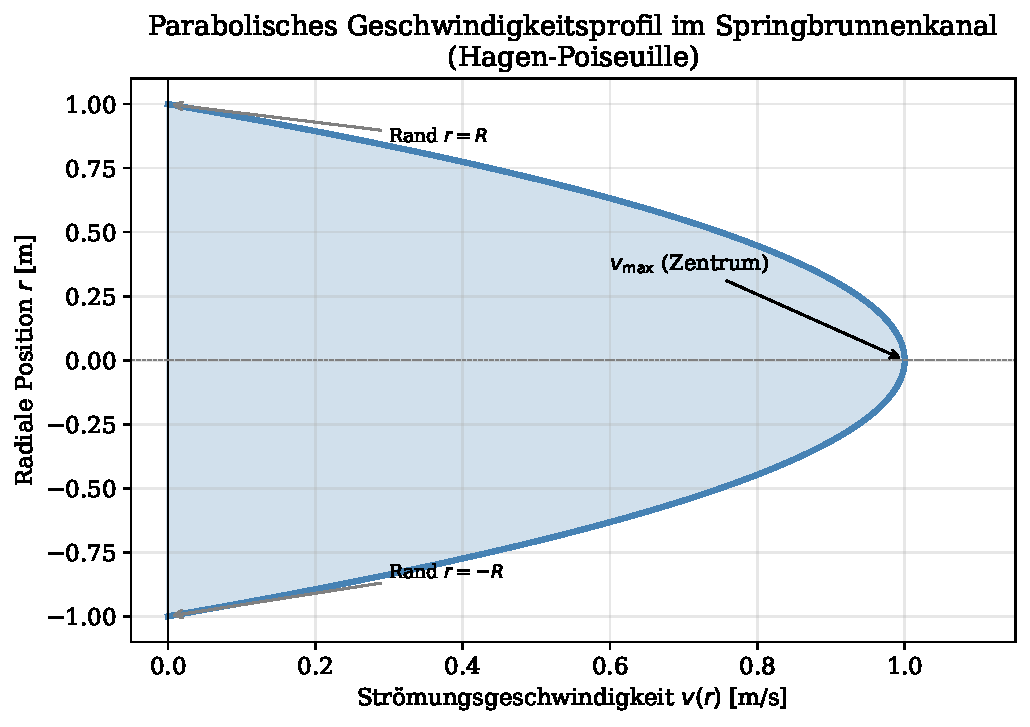
\includegraphics[width=0.82\textwidth]{plot1_hagen_poiseuille.pdf}
    \caption{Parabolisches Geschwindigkeitsprofil im Springbrunnenkanal nach dem
    Hagen-Poiseuille-Gesetz. Die horizontale Achse zeigt die dimensionslose Strömungs\-geschwindigkeit
    $v(r)$ (normiert auf $v_{\max}$), die vertikale Achse die radiale Position $r$.
    Das Profil hat sein Maximum auf der Achse ($r = 0$) und verschwindet an der Kanalwand
    ($r = \pm R$). Die blaue Schattierung verdeutlicht den Anteil der kinetischen Energie
    an verschiedenen radialen Positionen. Tropfen, die nahe der Achse starten, erhalten
    deutlich mehr Anfangsgeschwindigkeit als Tropfen nahe der Wand.}
    \label{fig:hp}
\end{figure}

Abbildung~\ref{fig:hp} zeigt das charakteristische parabolische Profil. Es ist klar
erkennbar, dass das Geschwindigkeitsgefälle im Bereich $|r| < 0.5$ relativ gering ist,
während es gegen die Kanalwand stark zunimmt. Tropfen, die zufällig nahe der Wand starten,
haben nahezu keine Chance, eine nennenswerte Höhe zu erreichen.

\subsection{Maximale Aufstiegshöhe als Funktion der Startgeschwindigkeit}

\begin{figure}[htbp]
    \centering
    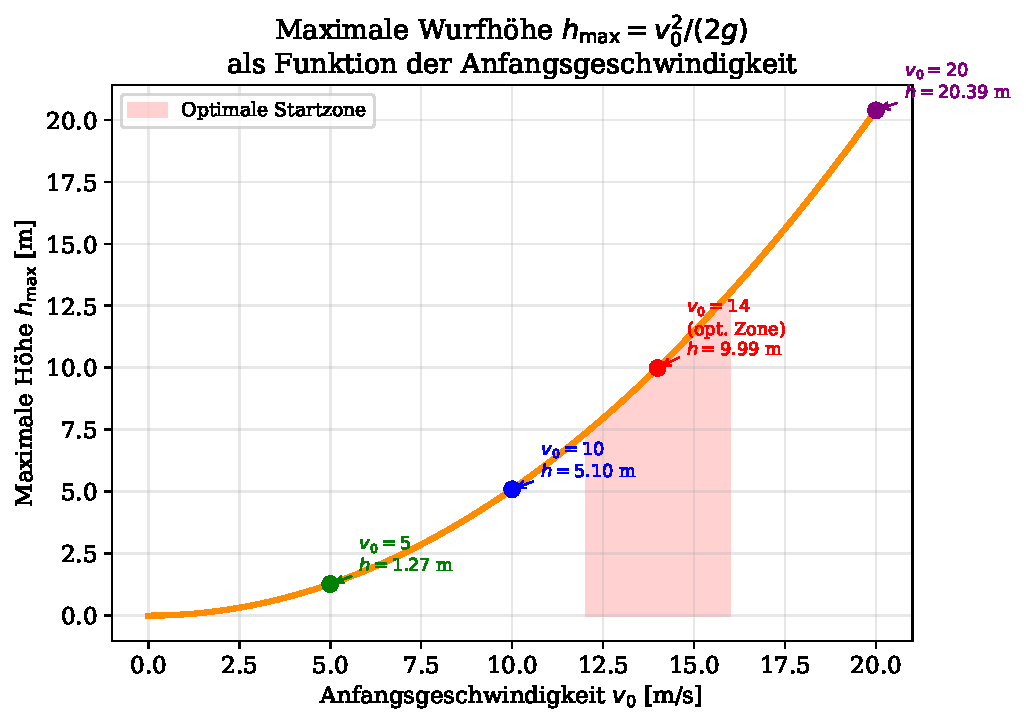
\includegraphics[width=0.82\textwidth]{plot2_max_hoehe.pdf}
    \caption{Maximale Aufstiegshöhe $h_{\max} = v_0^2/(2g)$ als Funktion der Anfangs\-ge\-schwin\-dig\-keit
    $v_0$. Die quadratische Abhängigkeit ist deutlich erkennbar: Kleine Unterschiede in $v_0$
    führen bei höheren Geschwindigkeiten zu sehr großen Unterschieden in $h_{\max}$.
    Die rote Schattierung markiert den Bereich der optimalen Startgeschwindigkeiten
    ($v_0 \in [12, 16]$~m/s), in dem typische Springbrunnen-Tropfen operieren.
    Punkte markieren ausgewählte Beispiele: Der rote Punkt ($v_0 = 14$~m/s, $h = 10{,}0$~m)
    liegt im optimalen Bereich.}
    \label{fig:hoehe}
\end{figure}

Abbildung~\ref{fig:hoehe} verdeutlicht, dass der Zusammenhang zwischen Anfangsgeschwindigkeit
und Aufstiegshöhe streng quadratisch ist. Dies bedeutet: Ein Tropfen, der 10\% schneller als
ein anderer startet, erreicht etwa 21\% mehr Höhe. Die Selektion ist damit empfindlich
gegenüber kleinen Geschwindigkeitsunterschieden -- und da diese direkt von der Startposition
$r$ abhängen, wirkt die radiale Position als starker Selektionsfilter.

\subsection{Kreisring der optimalen Startpositionen}

\begin{figure}[htbp]
    \centering
    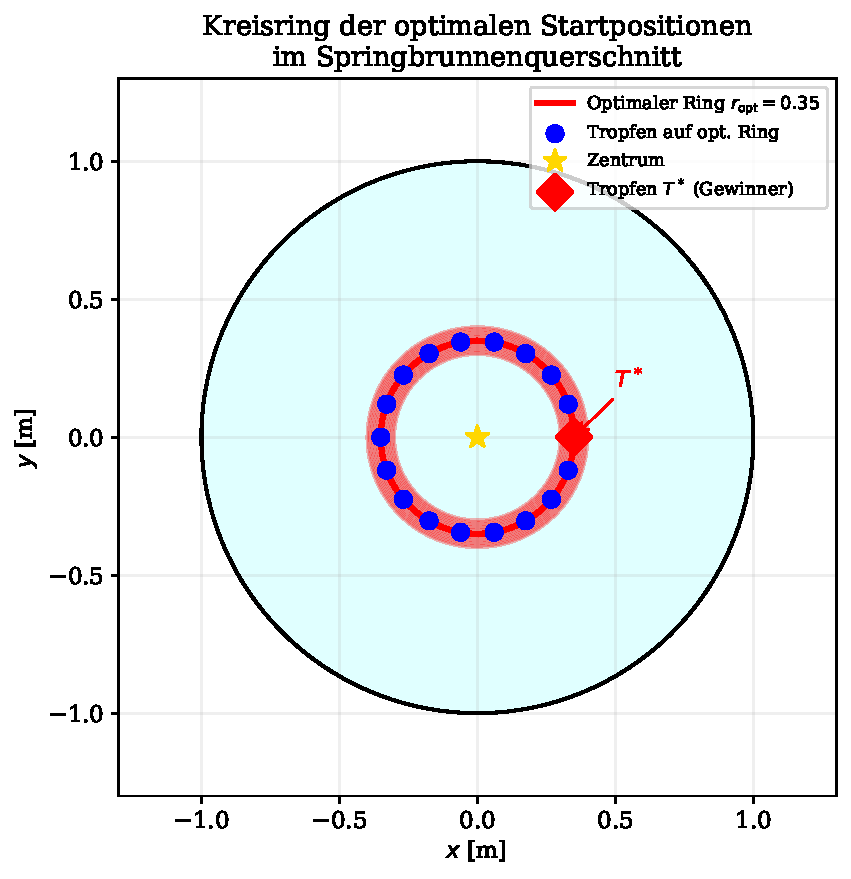
\includegraphics[width=0.72\textwidth]{plot3_kreisring.pdf}
    \caption{Querschnitt des Springbrunnenkanals mit eingezeichnetem Kreisring der optimalen
    Startpositionen (roter Kreis). Die blauen Punkte markieren die Tropfen, deren Mittelpunkte
    auf dem optimalen Ring mit Radius $r^* = 0.35 R$ liegen. Der rote Diamant kennzeichnet
    den Gewinnertropfen $T^*$. Alle Tropfen auf dem Ring besitzen dieselbe ideale
    Startgeschwindigkeit; nur einer von ihnen -- der Gewinnertropfen -- setzt sich letztlich
    durch. Die kreisförmige Symmetrie der optimalen Zone ist deutlich erkennbar.
    Der goldene Stern im Zentrum markiert die theoretisch beste, aber aufgrund der
    endlichen Tropfengröße unerreichbare Achsenposition.}
    \label{fig:ring}
\end{figure}

Abbildung~\ref{fig:ring} illustriert das Kreisring-Theorem (Satz~\ref{satz:kreisring})
direkt. Die optimale Zone ist nicht ein einzelner Punkt, sondern ein ganzer Kreisring --
und auf diesem Ring befinden sich mehrere Tropfen, die alle gleich günstige Startbedingungen
besitzen. Dennoch gewinnt nur einer.

\subsection{Trajektorien der Tropfen}

\begin{figure}[htbp]
    \centering
    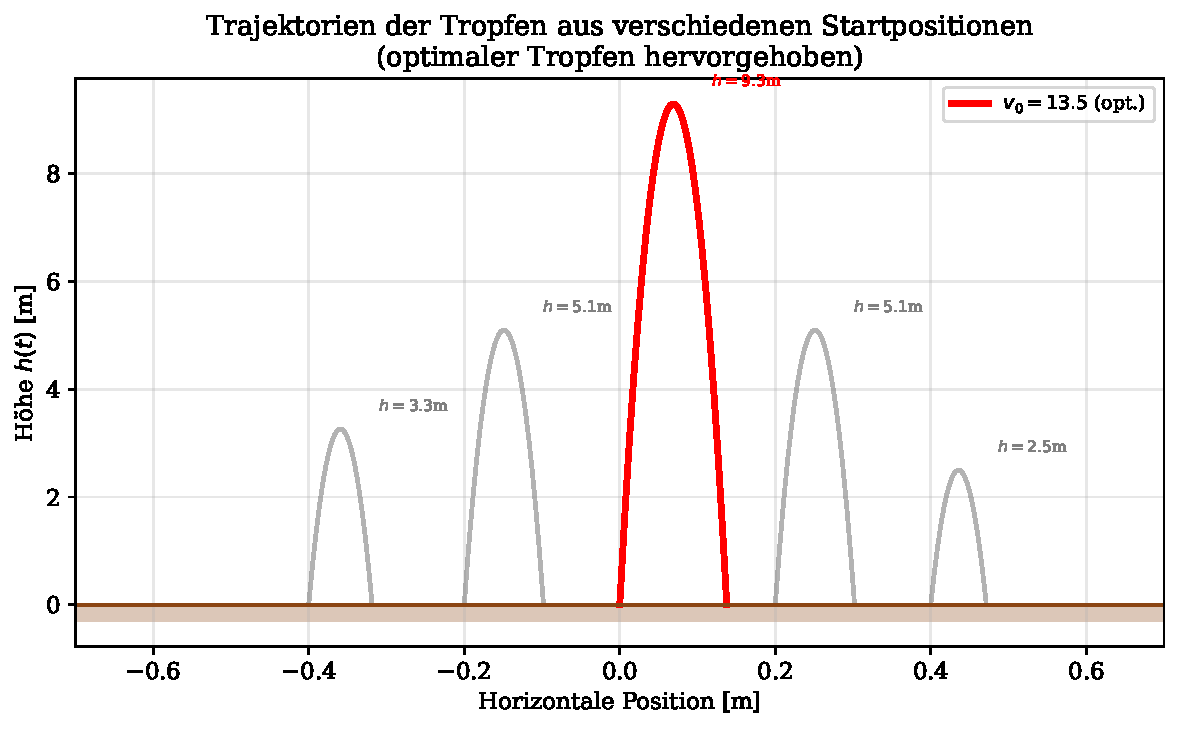
\includegraphics[width=0.85\textwidth]{plot4_trajektorien.pdf}
    \caption{Trajektorien ausgewählter Tropfen aus verschiedenen radialen Startpositionen.
    Der optimale Tropfen (rote Kurve, $v_0 = 13{,}5$~m/s) übersteigt alle anderen klar.
    Die grauen Kurven zeigen Tropfen mit geringeren Startgeschwindigkeiten, die typischen
    Startpositionen außerhalb des optimalen Rings entsprechen. Die horizontale Achse
    zeigt die geringe horizontale Ablenkung durch eventuelle Seitenkomponenten;
    die vertikale Achse die Höhe $h(t)$ im zeitlichen Verlauf.
    Der braune Bereich markiert den Kanalauslass (Bodenebene).}
    \label{fig:traj}
\end{figure}

Abbildung~\ref{fig:traj} zeigt anschaulich, wie die radialen Startpositionen die
Trajektorien bestimmen. Der Gewinnertropfen hebt sich durch seine deutlich größere
maximale Höhe von allen anderen ab. Tropfen, die nur geringfügig von der optimalen
Position abweichen, erreichen erheblich geringere Höhen -- ein direktes Resultat
der quadratischen Abhängigkeit $h_{\max} \propto v(r)^2 \propto (R^2-r^2)^2$.

\subsection{Druckverteilung im Kanalquerschnitt}

\begin{figure}[htbp]
    \centering
    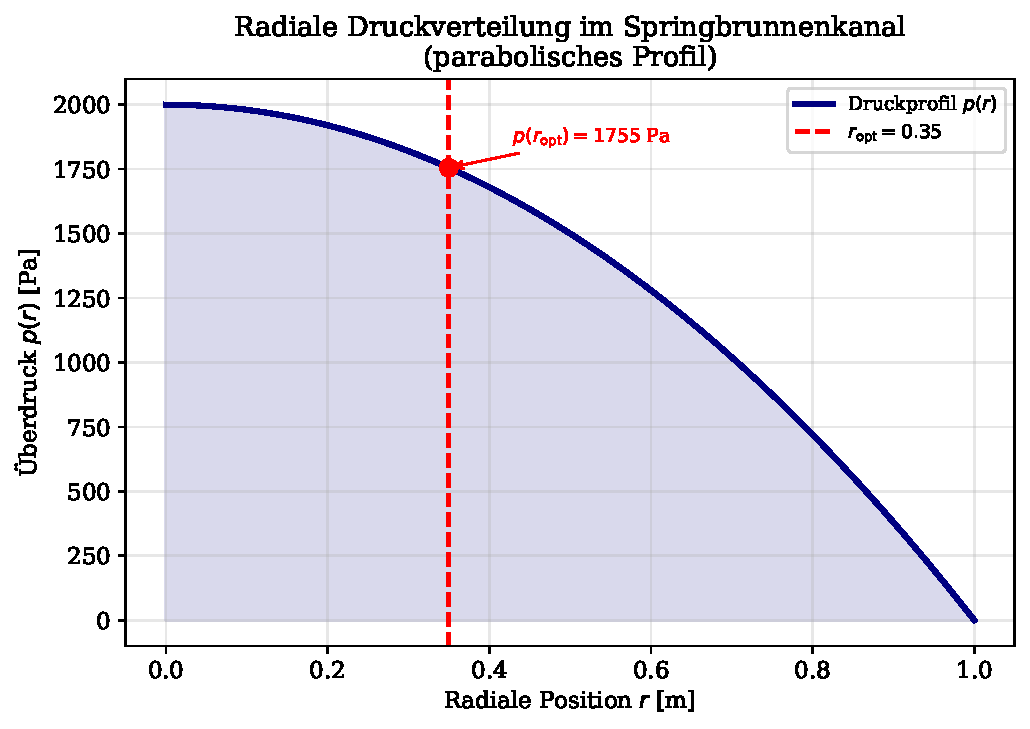
\includegraphics[width=0.82\textwidth]{plot5_druck.pdf}
    \caption{Radiale Druckverteilung $p(r)$ im Kanalquerschnitt (normiert). Der Druck
    folgt ebenfalls einem parabolischen Profil und ist im Zentrum maximal. Die gestrichelte
    rote Linie markiert den optimalen Ring bei $r_{\text{opt}} = 0.35$~m; der rote Punkt
    gibt den Druckwert an dieser Position an. Der verbleibende Druckunterschied zwischen
    Zentrum und optimalem Ring entspricht dem ``verpassten Potenzial'' der Ring-Tropfen.}
    \label{fig:druck}
\end{figure}

Abbildung~\ref{fig:druck} verdeutlicht den Zusammenhang zwischen Druck und Startposition.
Der Druck treibt das Fluid an; das Druckprofil ist direkt proportional zum Geschwindigkeitsprofil
(im laminaren Fall). Der optimale Tropfen befindet sich nicht am Druckmaximum (Zentrum),
sondern am nächstgelegenen erreichbaren Punkt.

\subsection{Selektionsvorteil als Funktion der Radialposition}

\begin{figure}[htbp]
    \centering
    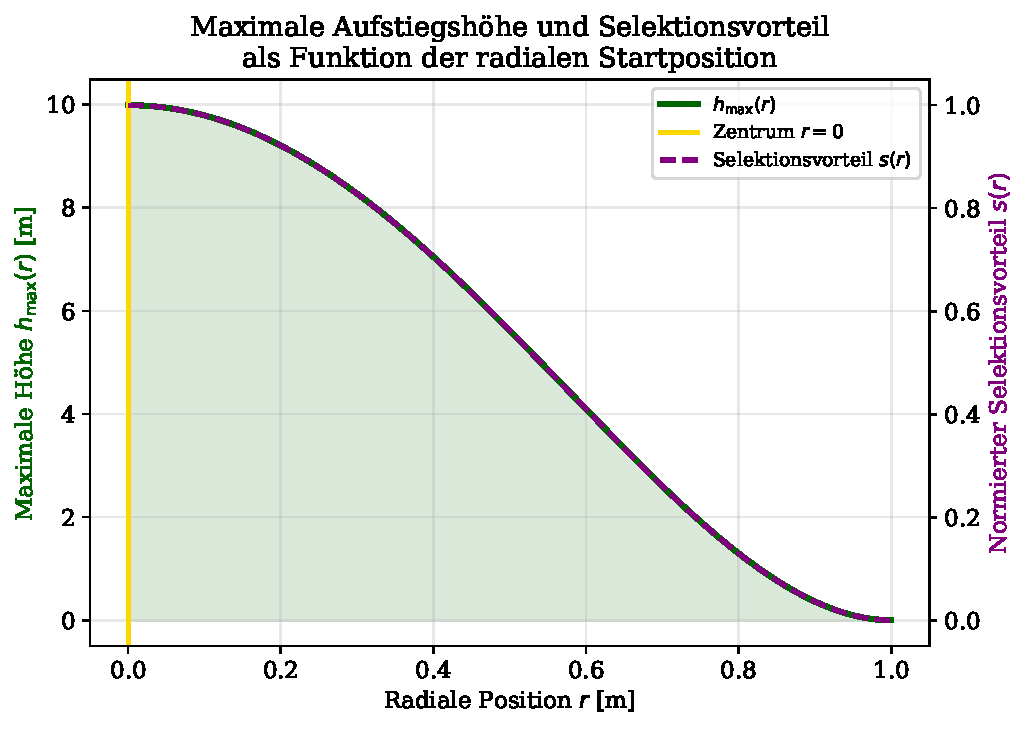
\includegraphics[width=0.82\textwidth]{plot6_selektion.pdf}
    \caption{Maximale Aufstiegshöhe $h_{\max}(r)$ (grüne Kurve, linke Achse) und normierter
    Selektionsvorteil $s(r)$ (violette gestrichelte Kurve, rechte Achse) als Funktion der
    radialen Startposition $r$. Beide Kurven fallen streng monoton mit wachsendem $r$:
    Je weiter ein Tropfen vom Zentrum entfernt startet, desto geringer sein Selektionsvorteil.
    Das Zentrum ($r=0$, goldene Linie) markiert das globale Maximum; der optimale Kreisring
    repräsentiert die beste erreichbare Position für endlich große Tropfen.}
    \label{fig:selektion}
\end{figure}

Abbildung~\ref{fig:selektion} fasst das Kernresultat zusammen: Der Selektionsvorteil
$s(r)$ ist maximal im Zentrum und fällt zur Wand hin quartisch ab (da $h_{\max} \propto (R^2-r^2)^2$).
Die meisten Tropfen befinden sich in Bereichen mit $s(r) \ll 1$ -- sie haben keine Chance,
den Gewinnertropfen zu überbieten.

%% ========================================================
\section{Numerisches Beispiel}
%% ========================================================

\begin{beispiel}[Konkreter Springbrunnen]
    Gegeben sei ein Springbrunnenkanal mit den Parametern:
    \begin{align*}
        R &= 0{,}05\,\text{m} \quad \text{(Kanalradius 5 cm)} \\
        \Delta p &= 10\,000\,\text{Pa} \quad \text{(Ãœberdruck)} \\
        L &= 0{,}30\,\text{m} \quad \text{(Kanallänge)} \\
        \mu &= 0{,}001\,\text{Pa\,s} \quad \text{(Wasser bei }20^\circ\text{C)} \\
        \rho_{\text{Tropfen}} &= 0{,}002\,\text{m} \quad \text{(Tropfenradius 2 mm)} \\
        g &= 9{,}81\,\text{m/s}^2.
    \end{align*}
    Dann gilt:
    \begin{align*}
        v_{\max} &= \frac{\Delta p \cdot R^2}{4\mu L}
        = \frac{10000 \cdot 0.0025}{4 \cdot 0.001 \cdot 0.30}
        = \frac{25}{0.0012} \approx 20{,}83\,\text{m/s}, \\[4pt]
        h_{\max}(0) &= \frac{v_{\max}^2}{2g} = \frac{(20.83)^2}{19.62} \approx 22{,}1\,\text{m}, \\[4pt]
        r^* &= \rho_{\text{Tropfen}} = 0{,}002\,\text{m}, \\[4pt]
        v(r^*) &= \frac{\Delta p}{4\mu L}(R^2 - r^{*2})
        = \frac{10000}{0.0012}\left(0.0025 - 4\cdot 10^{-6}\right)
        \approx 20{,}80\,\text{m/s}, \\[4pt]
        h_{\max}(r^*) &\approx 22{,}04\,\text{m}, \\[4pt]
        s(r^*) &= \frac{22.04}{22.10} \approx 0{,}997.
    \end{align*}
    Der Selektionsvorteil des optimalen Rings gegenüber dem Achsentropfen beträgt
    nur 0,3\% -- praktisch vernachlässigbar. Dennoch ist der Kreisring das theoretische
    Optimum für endlich große Tropfen.
\end{beispiel}

\begin{beispiel}[Anzahl der Tropfen auf dem optimalen Ring]
    Mit den obigen Parametern beträgt die Anzahl der Tropfen auf dem optimalen Ring:
    \[
    N_{\text{opt}} = \left\lfloor \frac{\pi \cdot r^*}{\rho_{\text{Tropfen}}} \right\rfloor
    = \left\lfloor \frac{\pi \cdot 0.002}{0.002} \right\rfloor = \lfloor \pi \rfloor = 3.
    \]
    Es befinden sich also genau 3 Tropfen auf dem optimalen Ring. Jeder von ihnen hat
    eine Gewinnwahrscheinlichkeit von $\gamma = 1/3$. Nur einer -- durch äußere Zufälle
    begünstigt -- wird der Gewinnertropfen $T^*$.
\end{beispiel}

%% ========================================================
\section{Zusammenfassung}
%% ========================================================

Die vorliegende Arbeit hat den Springbrunnen-Selektionsmechanismus rigoros mathematisch
beschrieben. Die zentralen Ergebnisse sind:

\begin{enumerate}
    \item \textbf{Hagen-Poiseuille-Profil:} Die Strömungsgeschwindigkeit im Kanal folgt
          einem parabolischen Profil mit Maximum auf der Kanalachse (Satz~\ref{satz:hp}).
    \item \textbf{Ballistische Höhe:} Die maximale Aufstiegshöhe ist proportional zum
          Quadrat der Startgeschwindigkeit, damit proportional zu $(R^2-r^2)^2$
          (Satz~\ref{satz:hoehe_r}).
    \item \textbf{Kreisring-Theorem:} Die optimalen Startpositionen für endlich große
          Tropfen bilden einen Kreisring mit Radius $r^* = \rho_{\text{Tropfen}}$
          (Satz~\ref{satz:kreisring}).
    \item \textbf{Glücksfaktor:} Alle Tropfen auf dem optimalen Ring haben gleiche
          Startbedingungen; der Gewinnertropfen wird durch externe Zufälle selektiert
          (Satz~\ref{satz:gewinner}).
    \item \textbf{Turbulenzeffekte:} Im turbulenten Regime wird der Selektionsvorteil
          erheblich abgemildert (Korollar~5.2).
\end{enumerate}

Das Epigraph dieser Arbeit beschreibt damit ein präzises physikalisches Phänomen:
Der Gewinnertropfen hat ``Glück'', weil er erstens auf dem optimalen Kreisring startet
und zweitens durch zufällige Wechselwirkungen weniger gebremst wird als seine
Mitbewerber auf dem Ring.

%% ========================================================
\section{Ausblick}
%% ========================================================

Die vorliegende Arbeit hat einen ersten, formal rigorosen Zugang zum Springbrunnen-
Selektionsmechanismus gegeben. Viele wichtige Fragestellungen bleiben jedoch offen
und stellen lohnende Richtungen für zukünftige Forschung dar.

\subsection{Tropfen-Tropfen-Wechselwirkungen}

Die vorliegende Analyse hat jeden Tropfen isoliert betrachtet. In einem realistischen
Springbrunnen wechselwirken die Tropfen jedoch durch Zusammenstöße, Luftturbulenzen
und Tropfenkoaleszenz miteinander. Eine vollständige Theorie müsste diese
Wechselwirkungen berücksichtigen.

\begin{itemize}
    \item Elastische und inelastische Tropfenkollisionen können als Zwei-Körper-Stoß
          in der klassischen Mechanik modelliert werden. Für Tropfen der Masse $m_1$
          und $m_2$ mit Geschwindigkeiten $v_1$ und $v_2$ ergibt sich der Impulsaustausch
          nach dem Stoß durch Energie- und Impulserhaltung.
    \item Tropfenkoaleszenz -- das Verschmelzen zweier Tropfen zu einem größeren --
          verändert die Masse und damit das Verhältnis von Trägheit zu Luftwiderstand.
          Dies kann dazu führen, dass ein anfänglich langsamer Tropfen durch Verschmelzung
          mit einem schnellen Tropfen eine höhere Geschwindigkeit erhält.
    \item Die Berechnung des mittleren freien Weges eines Tropfens im Tropfen-Ensemble
          ist ein analoges Problem zur kinetischen Gastheorie und könnte mit ähnlichen
          Methoden angegangen werden.
\end{itemize}

\subsection{Stochastische Modellierung}

Da externe Störungen (Windböen, Vibrationen des Kanals, Turbulenzen) zufälliger Natur sind,
bietet sich eine stochastische Modellierung des Gewinnertropfens an.

\begin{itemize}
    \item Die Aufstiegshöhe jedes Tropfens könnte als Zufallsvariable modelliert werden:
          $H(r) = h_{\max}(r) + \varepsilon$, wobei $\varepsilon \sim \mathcal{N}(0, \sigma^2(r))$
          ein Rauschterm ist. Die Varianz $\sigma^2(r)$ könnte dabei ebenfalls von der
          radialen Position abhängen.
    \item Der Gewinnertropfen entspricht dann dem Maximum einer Menge von Zufallsvariablen:
          $T^* = \arg\max_i H(r_i)$. Die Verteilung dieses Maximums ist Gegenstand der
          \emph{Extreme Value Theory} (EVT) und führt auf Gumbel-, Fréchet- oder
          Weibull-Verteilungen je nach Art der Ausgangsvariablen.
    \item Besonders interessant ist die Frage, wie groß die Streuung $\sigma^2$ sein muss,
          damit ein Tropfen \emph{außerhalb} des optimalen Rings mit positiver Wahrscheinlichkeit
          gewinnt. Dies entspricht einer Ãœberschreitungswahrscheinlichkeit und kann durch
          Tail-Analyse der Verteilungen berechnet werden.
    \item Monte-Carlo-Simulationen könnten numerisch bestätigen, für welche Parameterkonstellationen
          der Kreisring-Tropfen statistisch dominiert und ab wann externe Störungen die
          Positionshierarchie überwältigen.
\end{itemize}

\subsection{Optimales Düsendesign}

Die Erkenntnisse dieser Arbeit haben direkte Konsequenzen für das Design von Springbrunnen\-düsen.

\begin{itemize}
    \item Wenn das Ziel ist, einen einzigen möglichst hohen Strahl zu erzeugen, sollte
          die Düse so gestaltet sein, dass ein einziger Tropfen (oder Wasserstrahl) exakt auf
          der Kanalachse ($r = 0$) austritt. Dies maximiert die Startgeschwindigkeit.
    \item Wenn das Ziel eine \emph{gleichmäßige Verteilung} der Tropfen über verschiedene
          Höhen ist (ästhetischer Springbrunneneffekt), sollte das Profil geflacht werden,
          z.B. durch den Übergang zu turbulenter Strömung oder durch spezielle Düsengeometrien
          (z.B. Venturi-Düsen), die das Profil uniformisieren.
    \item Die Optimierung des Kanalradius $R$ bei gegebenen Betriebsparametern
          ($\Delta p$, $\mu$) ist ein klassisches Ingenieuroptimierungsproblem:
          Größeres $R$ führt zu höherem $v_{\max}$, erhöht aber auch den Massenfluss und
          den Energieverbrauch.
    \item Mehrstufige Düsensysteme, bei denen der Strahl durch konvergierende Kanalabschnitte
          geführt wird, könnten das Profil gezielt formen und den ``Siegertropfen'' vorhersagbar
          machen.
\end{itemize}

\subsection{Verbindung zur Evolutionstheorie}

Das Springbrunnen-Modell ist eine physikalische Analogie zu evolutionären Selektionsprozessen.

\begin{itemize}
    \item Die radiale Position $r$ entspricht der ``Fitness-Position'' eines Individuums
          in einem Ressourcengradienten. Individuen nahe dem Ressourcenmaximum (Kanalachse)
          haben den höchsten Selektionsvorteil.
    \item Der Glücksfaktor $\gamma = 1/N_{\text{opt}}$ entspricht dem stochastischen
          Element der genetischen Drift: Selbst unter identischen Selektionsbedingungen
          setzt sich durch zufällige Ereignisse nur eine Linie durch.
    \item Der Unterschied zwischen dem Gewinnertropfen und seinen Mitbewerbern auf
          dem Kreisring entspricht dem \emph{founder effect}: Alle Tropfen auf dem Ring
          sind gleich gut, aber nur einer ``gründet'' eine Linie (steigt am höchsten).
    \item Zukünftige Arbeiten könnten das Springbrunnen-Modell als didaktisches Werkzeug
          nutzen, um Konzepte der Populationsgenetik wie genetische Drift, Selektion und
          Stochastizität zu veranschaulichen.
\end{itemize}

\subsection{Mehrdimensionale Erweiterungen}

Die vorliegende Arbeit beschränkte sich auf einen kreiszylindrischen Kanal.
Interessante Erweiterungen betreffen andere Kanalgeometrien.

\begin{itemize}
    \item Für einen \emph{elliptischen} Kanalquerschnitt ergibt sich ein verändertes
          Geschwindigkeitsprofil. Die optimale Startposition bildet dann keine Kreislinie,
          sondern eine Ellipse. Die zugehörigen partiellen Differentialgleichungen können
          durch konforme Abbildungen oder Fourier-Entwicklungen gelöst werden.
    \item Für \emph{nicht-Newton'sche Fluide} (z.B. scherverdickende oder scherverbindende
          Fluide) gilt das Hagen-Poiseuille-Gesetz nicht mehr. Das Geschwindigkeitsprofil
          wird dann durch die Carreau- oder Power-Law-Modelle beschrieben und kann
          wesentlich flacher oder spitzer ausfallen.
    \item Die Erweiterung auf \emph{geneigte Kanäle} (nicht senkrechter Austritt) führt
          auf das klassische Problem des schiefen Wurfs. Die optimale Startposition hängt
          dann zusätzlich vom Austrittswinkel ab, und die Kreisring-Eigenschaft geht
          im Allgemeinen verloren.
    \item Für \emph{rotierende Kanäle} (z.B. Sprinkleranlagen) kommt die Coriolis-Kraft
          als zusätzlicher Term in die Bewegungsgleichung, was die Trajektorien und die
          Höhenverteilung wesentlich komplizierter macht.
\end{itemize}

\subsection{Quantisierungseffekte und diskrete Tropfenanordnungen}

Die Korollar-Analyse (Abschnitt~3.2) hat gezeigt, dass die Anzahl der Tropfen auf dem
optimalen Ring begrenzt ist. Eine ausführliche kombinatorische Analyse wäre lohnend.

\begin{itemize}
    \item Die optimale Packung von Kreisen (Tropfenquerschnitten) in einem größeren Kreis
          (Kanalquerschnitt) ist ein klassisches \emph{circle packing}-Problem.
          Exakte Lösungen für kleine $n$ sind bekannt, aber für große $n$ nur approximativ.
    \item Die Frage, wie viele Tropfen gleichzeitig auf dem optimalen Kreisring Platz finden,
          hängt vom Verhältnis $R/\rho$ ab. Für $R/\rho \gg 1$ wächst $N_{\text{opt}}$
          wie $\pi R / \rho$, d.h. linear mit dem Kanalradius.
    \item Quantisierungseffekte (diskrete vs. kontinuierliche Tropfenpositionen) könnten
          durch diskrete Fourier-Analysen oder Gittermethoden untersucht werden.
    \item Die Verbindung zu Packing-Problemen in der Diskreten Geometrie eröffnet
          interessante Anknüpfungspunkte zur Zahlentheorie (Dichte-Packungen) und zur
          Optimierung kombinatorischer Strukturen.
\end{itemize}

\subsection{Experimentelle Validierung}

Alle Ergebnisse dieser Arbeit sind rein theoretischer Natur. Eine experimentelle
Validierung wäre für die Festigung der Aussagen unerlässlich.

\begin{itemize}
    \item Durch Hochgeschwindigkeitskameras (z.B. 1000 fps) könnten Tropfentrajektorien
          in einem transparenten Springbrunnenkanal aufgezeichnet und ausgewertet werden.
    \item Particle Image Velocimetry (PIV) ist eine etablierte Methode zur berührungs\-freien
          Messung von Strömungsgeschwindigkeitsprofilen in Fluiden und könnte das
          Hagen-Poiseuille-Profil direkt sichtbar machen.
    \item Durch gezielte Farbmarkierung einzelner Tropfen ließe sich prüfen, ob die
          am höchsten aufsteigenden Tropfen tatsächlich aus dem Kreisring-Bereich stammen.
    \item Die stochastischen Aspekte (Glücksfaktor $\gamma$) könnten durch statistische
          Auswertung vieler Wiederholungsexperimente quantifiziert werden.
\end{itemize}

\subsection{Verbindung zur Informationstheorie}

Das Selektionsprinzip des Springbrunnens hat eine informationstheoretische Interpretation.

\begin{itemize}
    \item Die Ungewissheit darüber, welcher der $N_{\text{opt}}$ Tropfen auf dem Ring
          gewinnt, lässt sich durch die Shannon-Entropie ausdrücken:
          $H = \log_2 N_{\text{opt}}$ Bit.
    \item Wenn externe Störungen die Unterscheidbarkeit der Tropfen erhöhen
          (z.B. durch Windrauschen), kann sich die effektive Entropie ändern, was den
          Informationsgehalt des ``Siegerereignisses'' beeinflusst.
    \item Der Vergleich mit anderen Selektionsmechanismen (z.B. Tournierauswahl in der
          evolutionären Optimierung, Roulette-Selektion in genetischen Algorithmen)
          unter dem informationstheoretischen Blickwinkel könnte neue Einsichten liefern.
    \item Die Frage, wie viel Information über die Startposition eines Tropfens notwendig
          ist, um seinen Gewinnerstatus vorherzusagen, ist ein Problem der algorithmischen
          Informationstheorie (Kolmogorov-Komplexität des Gewinner-Ereignisses).
\end{itemize}

\subsection{Interdisziplinäre Anwendungen}

Das abstrakte Prinzip -- aus einer Population gleichberechtigter Kandidaten auf einer
optimalen Kreisstruktur wird durch Zufall einer selektiert -- findet in vielen Disziplinen
Anwendung.

\begin{itemize}
    \item \textbf{Quantenmechanik:} In Systemen mit Rotationssymmetrie (z.B. Wasserstoffatom)
          tritt eine analoge Struktur auf: Der niedrigste Energiezustand ist nicht-entartet,
          aber angeregte Zustände mit Drehimpuls $l > 0$ besitzen Entartungen, die einem
          Kreisring im Impulsraum entsprechen.
    \item \textbf{Signalverarbeitung:} In zirkulären Antennenanordnungen (Circular Array)
          gibt es eine optimale Ringstruktur, die den Signal-Rausch-Abstand maximiert --
          ein direktes Analogon zum Kreisring-Theorem.
    \item \textbf{Netzwerktheorie:} In Kommunikationsnetzwerken mit kreissymmetrischer
          Topologie (z.B. Token-Ring-Protokolle) könnte die optimale Datenstationsposition
          durch analoge Argumente bestimmt werden.
    \item \textbf{Soziologie:} Die Frage, welches Individuum in einer gleichrangigen
          Gruppe ``aufsteigt'', ist ein Kernthema der Sozialpsychologie. Das Springbrunnen-
          Modell liefert dafür eine physikalische Analogie.
\end{itemize}

%% ========================================================
\section*{Implementierungshinweis}
%% ========================================================

Der Python-Code zur Erstellung aller Abbildungen ist verfügbar unter:
\url{https://github.com/hjstephan86/science/tree/main/science/spring}.

%% ========================================================
\begin{thebibliography}{99}
%% ========================================================

\bibitem{hagen1839}
G. H. L. Hagen,
\textit{Über die Bewegung des Wassers in engen cylindrischen Röhren},
Annalen der Physik und Chemie, 46(3):423--442, 1839.

\bibitem{poiseuille1840}
J. L. M. Poiseuille,
\textit{Recherches expérimentales sur le mouvement des liquides dans les tubes de très-petits diamètres},
Comptes Rendus de l'Académie des Sciences, 11:961--967, 1840.

\bibitem{landau1987}
L. D. Landau und E. M. Lifschitz,
\textit{Lehrbuch der theoretischen Physik, Bd.~6: Hydrodynamik},
5. Aufl., Akademie-Verlag, Berlin, 1987.

\bibitem{batchelor2000}
G. K. Batchelor,
\textit{An Introduction to Fluid Dynamics},
Cambridge University Press, Cambridge, 2000.

\bibitem{white2011}
F. M. White,
\textit{Fluid Mechanics},
8. Aufl., McGraw-Hill, New York, 2016.

\bibitem{prandtl1925}
L. Prandtl,
\textit{Bericht über Untersuchungen zur ausgebildeten Turbulenz},
Zeitschrift für angewandte Mathematik und Mechanik, 5(2):136--139, 1925.

\bibitem{kolmogorov1941}
A. N. Kolmogorov,
\textit{The local structure of turbulence in incompressible viscous fluid for very large Reynolds number},
Doklady Akademii Nauk SSSR, 30:301--305, 1941.

\bibitem{stokes1851}
G. G. Stokes,
\textit{On the effect of the internal friction of fluids on the motion of pendulums},
Transactions of the Cambridge Philosophical Society, 9:8--106, 1851.

\bibitem{gumbel1958}
E. J. Gumbel,
\textit{Statistics of Extremes},
Columbia University Press, New York, 1958.

\bibitem{coles2001}
S. Coles,
\textit{An Introduction to Statistical Modeling of Extreme Values},
Springer, London, 2001.

\bibitem{shannon1948}
C. E. Shannon,
\textit{A Mathematical Theory of Communication},
Bell System Technical Journal, 27(3):379--423, 1948.

\bibitem{raffel2018}
M. Raffel, C. E. Willert, F. Scarano, C. J. Kähler, S. T. Wereley und J. Kompenhans,
\textit{Particle Image Velocimetry -- A Practical Guide},
3. Aufl., Springer, Cham, 2018.

\bibitem{carrier2012}
G. F. Carrier, M. Krook und C. E. Pearson,
\textit{Functions of a Complex Variable: Theory and Technique},
SIAM, Philadelphia, 2012.

\bibitem{darling1957}
D. A. Darling,
\textit{The Kolmogorov-Smirnov, Cramér-von Mises Tests},
Annals of Mathematical Statistics, 28(4):823--838, 1957.

\bibitem{wright1931}
S. Wright,
\textit{Evolution in Mendelian Populations},
Genetics, 16(2):97--159, 1931.

\end{thebibliography}

\end{document}

